\begin{savequote}[45mm]
The Theory of Relativity confers an absolute meaning on a magnitude which in classical theory has only a relative significance: the velocity of light. The velocity of light is to the Theory of Relativity as the elementary quantum of action is to the Quantum Theory: it is its absolute core.  
\qauthor{Max Planck}
\end{savequote}
\chapter{Preliminaries}
\label{ch:preliminaries}
\section{Special Relativity}
\begin{tcolorbox}
    Need for Special Relativity
\end{tcolorbox}
\begin{itemize}
    \item Newtonian Mechanics only seem to be relevant in certain frames of reference called as inertial frames of reference and all inertial frames of references are equivalent to each other. When we take up the case of Maxwell's theory of Electromagnetism, it was observed that there exists a set of preferred frames of references which goes against the understanding of the Galilean relativity. Hence to join the dots, Einstein formulated the theory of Special relativity which gives distinguished properties to individual frames of references wherein the speed of light is the only parameter that remains constant in all frames of reference.
    \item According to Special Relativity, the frames of reference are 4 dimensional. They are the spatial co-ordinate axes(x,y,z) and the time axis (t) and hence was termed as Space-time.
    \item Objects or "points" in a frame move along space and time and thus indicates that the events occurring in one frame need not occur in another frame at the same time.
    \item The points on a frame can be viewed on another frame of reference using some transformation laws. These transformation laws are called as Lorentz Transformation.
\end{itemize}
\subsection{Spacetime}
The distance between any two points in space is given by, 
\begin{equation}
    \Delta s^{2} = (\Delta x^{1})^{2} + (\Delta x^{2})^{2} + (\Delta x^{3})^{2} = \sum_{i=1}^{3}(\Delta x^{i})^{2}
\end{equation}
We can choose a new set of Cartesian axes and still the distance between the two points remain unchanged. 
\begin{equation}
\Delta s^{2} = \sum_{i=1}^{3}(\Delta x^{i^{1}})^{2}
\end{equation}
where the new set of axis is denoted by $x^{i^{1}}$. 
If the rotation between the axes is given by an angle $\theta$, we can  relate $x^{i}$ and $x^{i^{1}}$ by the equation, 
\begin{equation}
x^{i^{1}} = \Lambda ^{i^{1}} x^{i}_{i} =  \sum_{i=1}^{3} \Lambda ^{i^{1}} x^{i}_{i}
\end{equation}
\begin{equation}
x^{i^{1}} = \Lambda ^{i^{1}} x^{i}_{i}
\end{equation}
where, 
\begin{equation}
\Lambda ^{i^{1}} = \begin{pmatrix}
\cos \theta & \sin \theta & 0\\
-\sin \theta & \cos \theta & 0 \\
0 & 0 & 1
\end{pmatrix}
\end{equation}
Equation (1.4) gives the expression for Lorentz invariance.\\ 
In ordinary Newtonian physics, if one uses Cartesian coordinates, these are all the vector transformations one needs where the time variable 't' remains unchanged. \\
But it is not the case in Special Relativity. Special relativity refers to space-time and involves transformations that mix spacial co-ordinates and time co-ordinates together. 
\subsection{Minkowski Metric}
\begin{tcolorbox}
  \begin{equation}
     \Delta s^{2} = (c \Delta t)^{2} + (\Delta x^{1})^{2} + (\Delta x^{2})^{2} + (\Delta x^{3})^{2}
  \end{equation}
\end{tcolorbox}
The zeroth component in $x^{\mu}$ with $\mu = 0,1,2,3$ is the time component wherein it is expressed as 'ct' to keep the units of all the components same.Generally we take "c=1" to measure time in terms of distance. \\
The Lorentz invariant is given by, 
\begin{equation}
x^{\mu^{1}} = \Lambda ^{\mu ^{1}} x_{\mu} ^{\mu}
\end{equation}
For a rotation of the frame by an angle of $\theta$, we have the 
\begin{equation}
    \Lambda ^{\mu ^{1}}_{\mu} =  \begin{pmatrix}
1 & 0 & 0 & 0 \\
0 & \cos \theta & \sin \theta & 0\\
0 & -\sin \theta & \cos \theta & 0 \\
0 & 0 & 0 & 1 \\
\end{pmatrix}
\end{equation}
if we change to a coordinate system that is moving along the $x^{1}$ direction
with velocity v with respect to the original one, we have
\begin{equation}
    \Lambda ^{\mu ^{1}} _{\mu}  =  \begin{pmatrix}
\cos \phi & -\sin \phi & 0 & 0\\
-\sin \phi & \cos \phi & 0 & 0 \\
0 & 0 & 1 & 0 \\
0 & 0 & 0 & 1 \\
\end{pmatrix}
\end{equation}
where $\phi = tanh^{-1}(v) $ \\ 
Using the above expression, 
\begin{equation}
t^{1} = \gamma (t-vx)
\end{equation}
\begin{equation}
    x^{1} = \gamma (x-vt)
\end{equation} 
Where $\gamma = \frac{1}{\sqrt{1-v^{2}/c^{2}}}$ 
\subsection{Space-like, Time-like and Light-like}
\begin{tcolorbox}
\begin{itemize}
    \item At every point in space-time there is a future and past light cone 
    \item All points within the future or past light cones of a given point are said to be time-like separated with respect to a reference point and the space-time distance between those points is negative.
    \item Points outside the light cone are space-like separated and their distance to the origin is positive. 
    \item The points along the light cone are light-like or null separated and their distance to the origin is zero. 
\end{itemize}
 \end{tcolorbox}
 \subsection{Relativistic Mechanics}
 The proper length between two points in space-time is given by, 
 \begin{tcolorbox}
 \begin{equation}
    \Delta l = \int \sqrt{\eta_{{\mu}{\nu}} \frac{\delta x^{\mu}}{\delta \lambda} \frac{\delta x^{\nu}}{\delta \lambda} }\delta \lambda
 \end{equation}
 \end{tcolorbox}
 where $\lambda$ is a parameter of $x^{\mu}$ and ,
 \begin{equation*}
     \eta _{{\mu}{\nu}} = \Lambda_{\mu}^{\mu^{1}} \Lambda_{\nu}^{\nu^{1}} \eta _{{\mu^{1}}{\nu}^{1}}
 \end{equation*}
 The proper time for two events occurring at two different points in space-time is given by, 
 \begin{tcolorbox}
 \begin{equation}
  \Delta T = \int \sqrt{-\eta_{{\mu}{\nu}} \frac{\delta x^{\mu}}{\delta \lambda} \frac{\delta x^{\nu}}{\delta \lambda} }\delta \lambda
  \end{equation}
 \end{tcolorbox}
 The reason for the negative sign is that if we consider a space-time trajectory that does not move spatially, that is a particle at rest, then $\Delta T = \Delta t$ which is time measured at rest, with respect to the particle. Particle trajectories are always time-like or, if one considers massless particles, null. In that case the length of the trajectory disappears.
 \subsection{Raising and Lowering Indices}
 In space-time it is useful to make a distinction between sub-indices and super-indices. \\
 The four vectors $\eta_{\mu}^{\nu}$ and  $\eta_{\nu}^{\mu}$ are not one and the same. \\
 We can define the four vectors with different indices with the expression, 
 \begin{equation}
  \eta_{\mu} = \Lambda^{{\mu}{\nu}} \eta^{\nu}
 \end{equation}
 and for the other case, 
 \begin{equation}
     \eta^{\mu} = \Lambda_{{\mu}{\nu}} \eta_{\nu}
 \end{equation}
 This is called lowering or raising indices which will prove essential for formulating the expressions for various other four vectors. 
 \section{An example: Compton Effect}
 
 Lets try applying the four vector formulism to a very renowned formula based on Compton effect. \\
 The 4-momentum of a particle is given by ,
 \begin{equation}
    P \equiv (P_{0}, P_{1}, P_{3}, P_{4}) \equiv (E, P_{x}c, P_{y}c, P_{z}c) \equiv (E, pc)
 \end{equation}
 The square of a 4-momentum that is, the inner product of a 4-momentum with
itself is therefore,
\begin{equation}
    P^{2} \equiv P . P \equiv E^{2} - |P|^{2}c^{2}= m^{2}c^{4}
\end{equation}
Since momentum in conserved, the initial momentum is equal to the momentum after collision. $P_{initial}= P_{final}$ \\

The 4-Momenta before the collision is given by,
\begin{equation}
    P_{initial} = (\frac{hc}{\lambda}, \frac{hc}{\lambda}, 0, 0) , \: P_{m} = (mc^{2}, 0, 0, 0)
\end{equation}
The 4-Momenta before the collision is given by,
\begin{equation}
   P_{final} = (\frac{hc}{\lambda^{1}}, \frac{hc}{\lambda^{1}} \cos{\theta}, \frac{hc}{\lambda^{1}} \sin{\theta}, 0) 
\end{equation}
 
 \begin{figure}
    \centering
    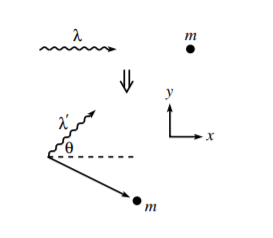
\includegraphics{Figures/compton effect .png}
    \caption{Compton Scattering}
    \label{fig:my_label}
\end{figure}
From the law of conservation of momentum and energy,  we get, 
\begin{eqnarray}
P_{initial} + P_{m} = P_{final}+ P_{m}^{1} \\
(P_{initial} + P_{m}- P_{final})^{2}  = (P_{m}^{1})^{2} \\
P_{initial}^{2} + P_{m}^{2}+ P_{final}^{2} + 2 P_{m}(P_{initial} - P_{final} )- 2 P_{initial}P_{final} = (P_{m}^{1})^{2} \\
0+ m^{2}c^{4} + 0 + 2m c^{2}(\frac{hc}{\lambda} -\frac{hc}{\lambda^{1}}) - 2 \frac{hc}{\lambda} \frac{hc}{\lambda^{1}} (1-\cos{\theta}) = m^{2}c^{4}
\end{eqnarray}
Multiplying throughout by $(\frac{\lambda \lambda^{1}}{2hmc^{3}})$ f=gives, 
\begin{equation}
    \lambda^{1} = \lambda + \frac{h}{mc}(1- \cos{\theta})
\end{equation}
\begin{itemize}
    \item If $\theta \approx 0$, then $\lambda \approx \lambda^{1}$
    \item if $\\theta = \pi $ and $\lambda << \frac{h}{mc} $ then, $\lambda^{1}= \frac{2h}{mc}$, so, 
    \begin{equation}
    E_{final}=\frac{hc}{\lambda} \approx \frac{\frac{hc}{2h}}{mc} = \frac{1}{2}mc^{2}
    \end{equation}
    That is to say that the photon bounces back with a certain $E_{final}$ which is independent of $E_{initial}$. 
\end{itemize}


